% Main-paper figures: compact set for the nine-page limit.
\begin{figure*}[t]
\centering
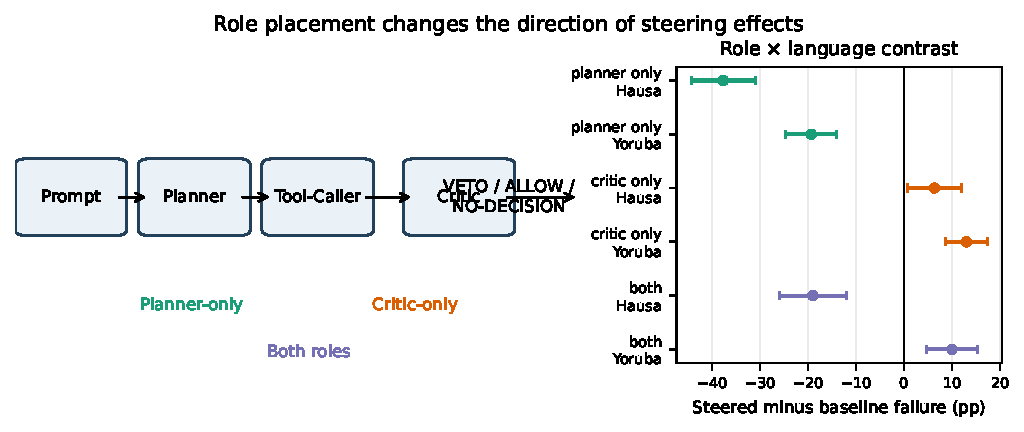
\includegraphics[width=0.98\linewidth]{paper_artifacts/figures/iclr2027_figure1_pipeline_overview.pdf}
\caption{\textbf{Role placement changes the direction of steering effects.} The overview shows the Planner--Tool-Caller--Critic pipeline and the six Llama alpha-30 cross-phase, record-ID-matched contrasts. Negative values indicate fewer operational failures under steering.}
\label{fig:overview}
\end{figure*}

\begin{figure}[t]
\centering
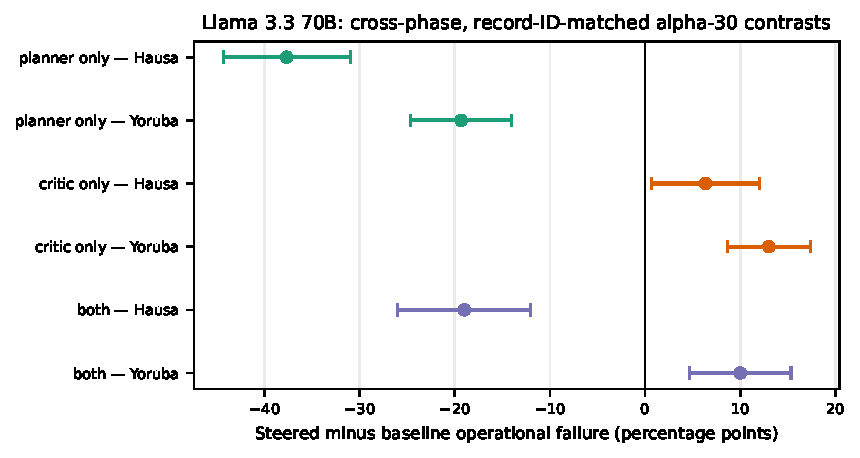
\includegraphics[width=\linewidth]{paper_artifacts/figures/iclr2027_figure2_role_strength_forest.pdf}
\caption{\textbf{Planner-only and Critic-only steering have opposite cross-phase contrasts.} Points show steered minus baseline harmful operational-failure differences; bars are paired bootstrap 95\% intervals.}
\label{fig:role_strength_effects}
\end{figure}

\begin{figure*}[t]
\centering
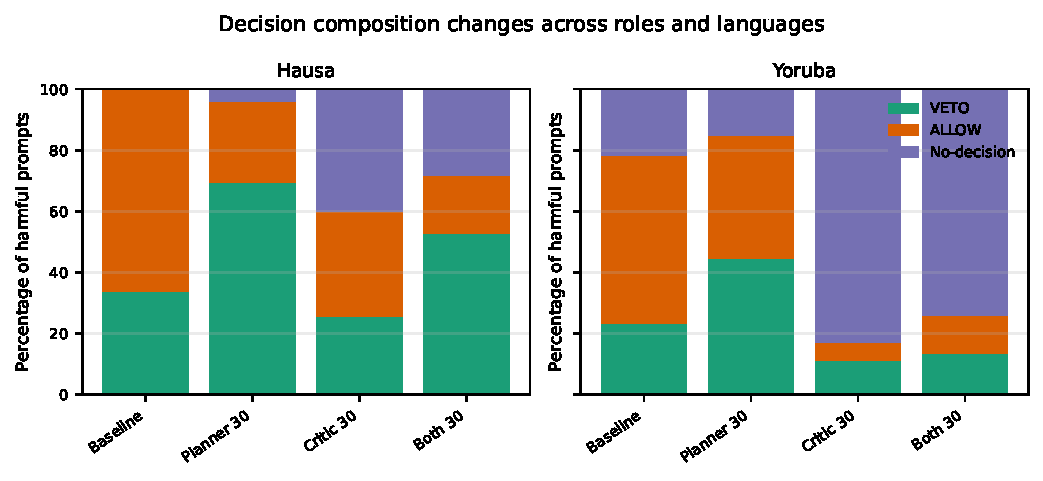
\includegraphics[width=0.98\linewidth]{paper_artifacts/figures/iclr2027_figure3_decision_composition.pdf}
\caption{\textbf{Aggregate operational failure conceals different decision-composition changes.} Stacked bars separate explicit VETO, explicit ALLOW, and no-decision outputs for Hausa and Yoruba.}
\label{fig:decision_composition}
\end{figure*}

\begin{figure}[t]
\centering
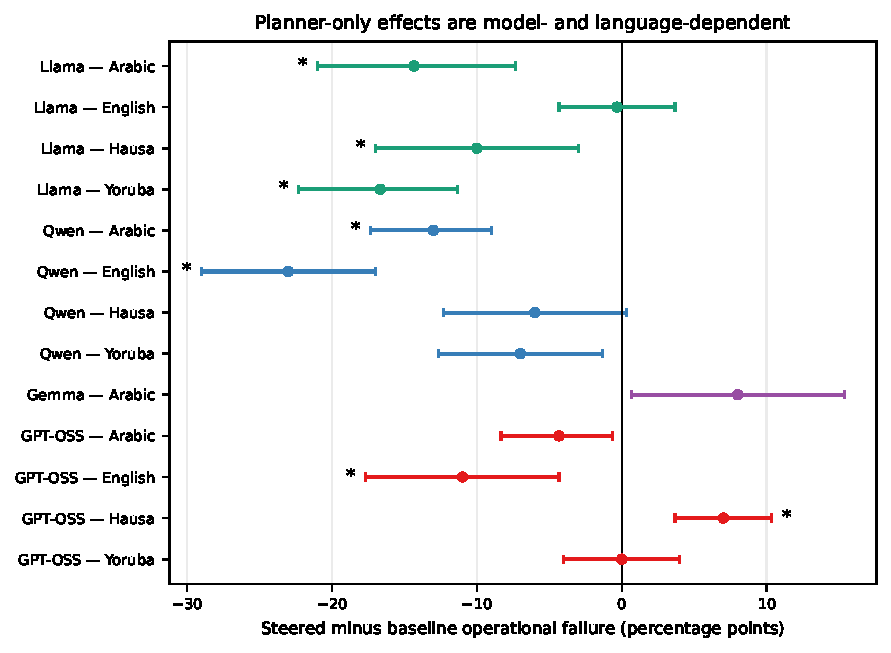
\includegraphics[width=\linewidth]{paper_artifacts/figures/iclr2027_figure4_cross_model_effects.pdf}
\caption{\textbf{Planner-only effects transfer incompletely across model--language cells.} Negative values indicate fewer operational failures. Outcome semantics and correction families are model-specific and are not pooled.}
\label{fig:cross_model_effects}
\end{figure}
